\documentclass[a4,12pt]{article}

%--- Packages génériques ---%

\usepackage[english]{babel}
\usepackage[utf8]{inputenc}
\usepackage[T1]{fontenc}
\usepackage[babel=true]{csquotes}
\usepackage{amsmath}
\usepackage{amssymb}
\usepackage{textcomp}
\usepackage{float}
\usepackage{graphicx}
\usepackage{caption}
\usepackage{hyperref}
\usepackage{empheq}
\usepackage{color}
\usepackage{cancel}
\usepackage{textcomp} %% pour les intervalles d'entiers(doubles barres)

%--- Structure de la page ---%

\usepackage{fancyheadings}

\topmargin -1.5 cm
\oddsidemargin -0.5 cm
\evensidemargin -0.5 cm
\textwidth 17 cm
\setlength{\headwidth}{\textwidth}
\textheight 24 cm
\pagestyle{fancy}
\lhead[\fancyplain{}{\thepage}]{\fancyplain{}{\sl MSIAM 3A}}
\chead[\fancyplain{}{{\sl }}]{\fancyplain{}{{Summary}}}
\rhead[\fancyplain{}{}]{\fancyplain{}{Mazouth--Laurol}}
\lfoot{\fancyplain{}{}}
\cfoot{\fancyplain{}{}}
\cfoot{\thepage }
\rfoot{\fancyplain{}{}}

%--- Raccourcis commande ---%

\newcommand{\R}{\mathbb{R}}
\newcommand{\N}{\mathbb{N}}
\newcommand{\A}{\mathbf{A}}
\newcommand{\B}{\mathbf{B}}
\newcommand{\C}{\mathbf{C}}
\newcommand{\D}{\mathbf{D}}
\newcommand{\ub}{\mathbf{u}}

\DeclareMathOperator{\e}{e}
%--- Header to write code ---%
\usepackage { listings }
%%configuration de listings
\lstset{
	language=c++,
	basicstyle=\ttfamily\small, %
	identifierstyle=\color{black}, %
	keywordstyle=\color{blue}, %
	stringstyle=\color{black!60}, %
	commentstyle=\it\color{green!95!yellow!1}, %
	columns=flexible, %
	tabsize=2, %
	extendedchars=true, %
	showspaces=false, %
	showstringspaces=false, %
	numbers=left, %
	numberstyle=\tiny, %
	breaklines=true, %
	breakautoindent=true, %
	captionpos=b
}


\usepackage{xcolor}


\definecolor{Zgris}{rgb}{0.87,0.85,0.85}


\newsavebox{\BBbox}
\newenvironment{DDbox}[1]{
	\begin{lrbox}{\BBbox}\begin{minipage}{\linewidth}}
		{\end{minipage}\end{lrbox}\noindent\colorbox{Zgris}{\usebox{\BBbox}} \\
	[.5cm]}
%--- Mode correction et incréments automatiques ---%

\usepackage{framed}
\usepackage{ifthen}
\usepackage{comment}

\newcounter{Nbquestion}

\newcommand*\question{%
\stepcounter{Nbquestion}%
\textbf{Question \theNbquestion. }}

\newboolean{enseignant}
%\setboolean{enseignant}{true}
\setboolean{enseignant}{false}

\ifthenelse{
\boolean{enseignant}}{
\newenvironment{correction}{\begin{shaded}}{\end{shaded}}
}
{
\excludecomment{correction}
}

%%%%%%%%%%%%%%%%%%%%%%%%%%%%%%%%%%%%%%%%%%%%%%%%%%%%%%%%
% 							               EN-TETE        

\title{\textbf{Tomography reconstruction from 2D projections}}
\author{
\begin{tabular}{cc}
	\textsc{Maxime Mazouth--Laurol}
\end{tabular}}   
\date{\small $8^{th}$ January 2018}

\makeatletter
	\def\thetitle{\@title}
	\def\theauthor{\@author}
	\def\thedate{\@date}
\makeatother 

\usepackage{etoolbox}
\usepackage{titling}
\setlength{\droptitle}{-7em}

\setlength{\parindent}{0cm}

\makeatletter
% patch pour le bug concernant les parenthèses fermantes d'après http://tex.stackexchange.com/q/69472
\patchcmd{\lsthk@SelectCharTable}{%
  \lst@ifbreaklines\lst@Def{`)}{\lst@breakProcessOther)}\fi}{}{}{}
\begin{document}

\maketitle
\paragraph{Reminder}
~~ So far, the work was about highlighting sinograms for basic  images thanks to complete parallel projections, and verifying well-known Helgason-Ludwig conditions. For now, the aim of the project is to emphasize new DCC applicable directly on truncated projections. Thus, we are first concerned here with retrieving truncated data, then using them to check this new DCC described below : \\
\[
p = \Re f ~ \text{for some density function }f \Leftrightarrow B_{n}(x) = \int_{-\frac{\pi}{2}}^{\frac{\pi}{2}}p(\phi,x\cos\phi + y0\sin\phi)\frac{\tan^{n}\phi}{\cos\phi}d\phi
\] is a polynomial of degree n. This is supposed to be true for the line $y=y0$ well-positioned as described in\cite{truncProj}

\section{Results}
~~ Hence, for a framework looking-alike the one provided in the document, consistent results are derived, attesting the truth of the mathematical property of $B_n$, for n $\in \mathbb{N}$.

\begin{figure}[h!]
   \begin{minipage}[c]{.46\linewidth}
      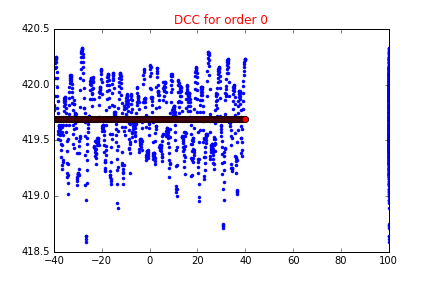
\includegraphics[scale=0.5]{../images/dcc/DCC0.png} 
      \captionof{figure}{DCC Order 0}
   \end{minipage} \hfill
   \begin{minipage}[c]{.46\linewidth}
      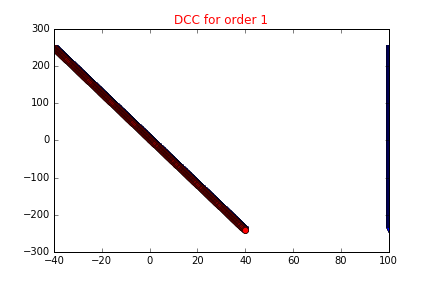
\includegraphics[scale=0.5]{../images/dcc/DCC1.png} 
      \captionof{figure}{DCC Order 1}
   \end{minipage}
\end{figure}

\begin{figure}[h!]
   \begin{minipage}[c]{.46\linewidth}
      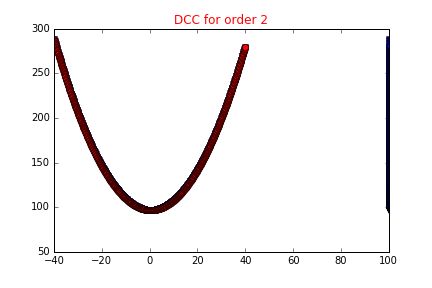
\includegraphics[scale=0.5]{../images/dcc/DCC2.png} 
      \captionof{figure}{DCC Order 2}
   \end{minipage} \hfill
   \begin{minipage}[c]{.46\linewidth}
      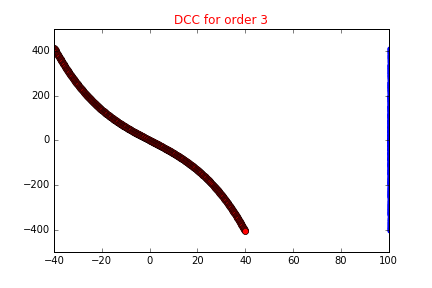
\includegraphics[scale=0.5]{../images/dcc/DCC3.png} 
      \captionof{figure}{DCC Order 3}
   \end{minipage}
\end{figure}

The polynomial approximation is a \textbf{least square polynomial fit}, obtained with \verb!numpy.polyfit! function. \\ \\
There is no analysis of these results yet, but one can notice how accurate this approximation is with respect to the $B_n$ values, which looks positive for now. 
\newpage

\bibliographystyle{plain}
\bibliography{reportPerso1}
\end{document}